%Chassis
\subsection{Introduction}
%~~~~~~~~~~~~~~~~~~~~~~~~~~~~~~~~~~~~~~~~~~~~~~~~~~~~~~~~~~~~
L'opération châssis n'a débuté qu'après avoir défini avec toute l'équipe quelles actions le robot devra accomplir. La décision s'est prise principalement en fonction du nombre de points que cela pourrait nous rapporter en tenant compte de la complexité demandée et du temps que celle-ci demande. 

\paragraph{}
Ensemble, nous avons donc conclu qu'une pince était amplement suffisante pour réaliser 3 des 5 actions demandés pour le concours. Cette année nous avons décidé d'utiliser deux robots pour répondre à nos besoins : un robot avec un mécanisme élévateur composé de la pince et un robot chenille. Les actions définies, nous avons pu mettre en place les techniques choisies pour les accomplir.

\subsection{Objectifs}
%~~~~~~~~~~~~~~~~~~~~~~~~~~~~~~~~~~~~~~~~~~~~~~~~~~~~~~~~~~~~
Conception d'une base adéquate capable de recevoir une pince mécanique et les nouveaux moteurs acquis cette année. 

\paragraph{}
La pince mécanique doit être capable de soulever un objet, de le transporter à un endroit souhaité et d'empiler des objets les uns sur les autres.

\subsection{Étude de l'existant}
%~~~~~~~~~~~~~~~~~~~~~~~~~~~~~~~~~~~~~~~~~~~~~~~~~~~~~~~~~~~~
Après une étude et un choix de ce qui est à notre disposition. Nous avons décidé de nous baser sur le principe du mécanisme d'élévation présent sur un châssis déjà monté afin d'assurer le déplacement vertical de la pince. Malheureusement, ce châssis ne peut être réutilisé vu qu'il n'appartient pas à l'ECAM.

\paragraph{}
L'autre châssis, celui de l'ECAM n'est plus adéquat avec ce que l'on a besoin étant donné que les nouveaux moteurs ont été dimensionnés avec le réducteur adéquat ce qui allonge l'emplacement du support moteur.

\subsection{Mécanisme d'élévation}
%~~~~~~~~~~~~~~~~~~~~~~~~~~~~~~~~~~~~~~~~~~~~~~~~~~~~~~~~~~~~
L'élévation sera donc assurée par un rail constitué d'un guidage et d'une poulie à chacune de ces extrémités dont la liaison est assurée par une courroie crantée contrôlée par un servomoteur. Une pièce métallique est attachée à la courroie et assure le déplacement de la pince.  

\noindent On peut voir à la figure~\ref{fig:Chariot} un élément représentatif qui a été réalisé sous CATIA.

\begin{figure}[!ht]
	\centering
		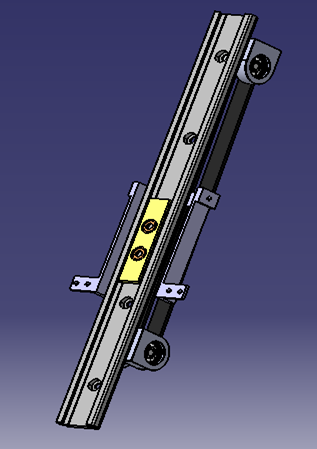
\includegraphics{chariot.png}
	\caption{Mécanisme d'élévation}
	\label{fig:Chariot}
\end{figure}

\noindent Ce mécanise correspondait bien avec ce dont on a besoin comme par exemple :  

\begin{itemize}
	\item Montée à la hauteur de 200mm pour atteindre le distributeur de pop-corn;
	\item Ou encore monter à plus de 210mm afin d'empiler par exemple 3 pieds et placer une balle de tennis pour réaliser le spot de lumière.
\end{itemize}

\paragraph{}
Ainsi nous sommes partis sur ce principe et avons réalisé une base prévue pour recevoir le mécanisme d'élévation, notamment la pince dont les servomoteurs seront implémentés de manière à se retrouver à l'intérieur de la surface totale du châssis. Ceci est nécessaire afin de minimiser la longueur totale du robot et d'éviter que la pince ressorte trop vers l'extérieur à cause de la présence des servomoteurs.

\subsection{Support moteur}
%~~~~~~~~~~~~~~~~~~~~~~~~~~~~~~~~~~~~~~~~~~~~~~~~~~~~~~~~~~~~
Pour la mise en place du moteur, nous avons totalement changé le système d'accouplement de la roue au moteur par rapport aux années précédentes. Nous avons choisi l'option la plus simple c'est-à-dire lier le moteur a la roue directement sans passer par la courroie et la poulie de réduction, étant donné qu'un réducteur existe déjà dans le moteur.

\paragraph{}
La seule pièce qu'on a dû créer est le support du moteur (figure~\ref{fig:support}) vu que la fixation du moteur sur le support exige une grande précision en tenant compte des tolérances, nous nous sommes basés  sur une pièce déjà existante. En la modifiant, nous avons créé un système simple pour la mise en place des moteurs et en même temps solide, surtout que le moteur présente un couple élevé après l'étage de réduction de la vitesse.

\begin{figure}[!ht]
	\centering
		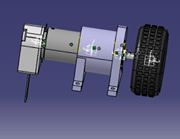
\includegraphics{support.jpg}
	\caption{Support Moteur}
	\label{fig:support}
\end{figure}

\subsection{Assemblage des différents éléments}
%~~~~~~~~~~~~~~~~~~~~~~~~~~~~~~~~~~~~~~~~~~~~~~~~~~~~~~~~~~~~
Afin de mieux visualiser la longueur totale de notre robot et de minimiser l'emplacement, un modèle de notre robot a été réalisée sous CATIA.

\vspace{5mm}
\begin{figure}[!ht]
	\centering
		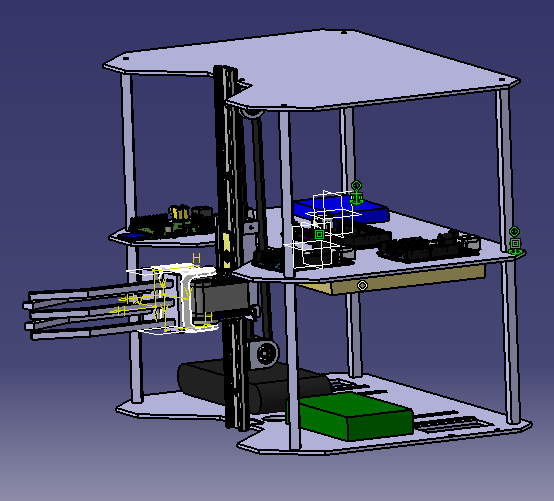
\includegraphics{assemblage.png}
	\caption{Éléments assemblés}
	\label{fig:assemblage}
\end{figure}

\paragraph{}
Le châssis du robot qui sera construit en P2 sera constitué de 2 plaques :
\begin{itemize}
	\item La base qui sera réalisée en aluminium sera composée des éléments comme le moteur, la batterie et le driver; 
	\item La deuxième plaque sera réalisée soit en PVC soit en aluminium, celle-ci sera constituée de toutes les cartes comme l'alimentation (partie d'en dessous) la Raspberry Pi, Arduino Mega, Arduino Uno et DE0-nano.
\end{itemize}

\paragraph{}
La réalisation de la pince a été entreprise par Nehri Nabil en même temps que la réalisation de la base. La création des supports pour les cartes électroniques n'a pas encore été réalisée notamment dû à l'incertitude de l'emplacement définitif des cartes. 

\paragraph{}
À ce stade, nous ne savons pas si de nouvelles cartes électroniques peuvent encore être créées ou modifiées. Le positionnement sera ajusté par étape d'implémentation en P2.

\noindent Le robot présente approximativement comme valeurs maxima une longueur de 240mm sans la pince et 370mm si on tient compte de celle-ci. Il fait également 340mm de largeur contre un peu plus de 300mm de hauteur.

\subsubsection{Inconvénients}
\begin{itemize}
	\item On ne peut faire qu'une action à la fois car 3 actions dépendent de la pince;
	\item Peut présenter un souci pour se positionner face à un objet à cause des capteurs qui doivent être présents pour assurer son positionnement;
	\item  La pince demande deux servomoteurs qui rendent les commandes plus difficiles mais offrent un meilleur résultat;
	\item L'encombrement de la pince est de 170mm de longueur ce qui est un handicap, elle augmente considérablement la taille du robot.
\end{itemize}

\subsection{Problèmes rencontrés}
%~~~~~~~~~~~~~~~~~~~~~~~~~~~~~~~~~~~~~~~~~~~~~~~~~~~~~~~~~~~~
Le principal souci rencontré a été que si l'on utilise une version supérieure de CATIA, il devient impossible d'ouvrir un fichier d'une version antérieure. Malheureusement, nous nous sommes rendus compte de ceci une fois la mise en commun des différentes réalisations.

\subsection{Annexes}
%~~~~~~~~~~~~~~~~~~~~~~~~~~~~~~~~~~~~~~~~~~~~~~~~~~~~~~~~~~~~
Tout les plans, ainsi que toutes les réalisations avec CATIA se trouvent dans le dossier Éléments CATIA déposé sur silicium.